\documentclass[tikz,border=8pt]{standalone}
\usepackage{bm,amsmath}
\usetikzlibrary{arrows.meta, positioning, calc}

\begin{document}
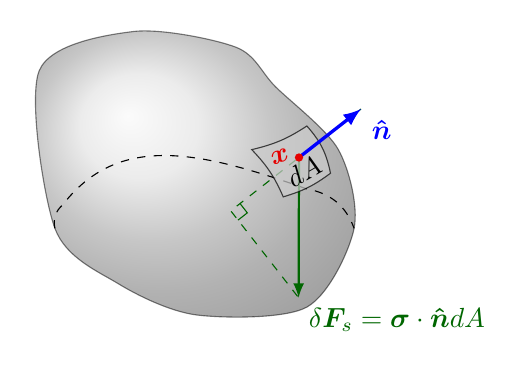
\begin{tikzpicture}
\usetikzlibrary{calc}
\shadedraw[ball color=gray!40,opacity=0.5] plot[smooth cycle] coordinates {(-2,1) (-0.8,1.5) (0.5,1.3) (1,0.8) (1.8,0) (2,-1) (1.4,-2) (0,-2.1) (-1,-1.7) (-1.8,-1)};
\draw[dashed] (-1.8,-1) to[bend left=30] (-1.7,-0.7) .. controls (-1,0.2) and (0,0) .. (1.4,-0.5) to [bend left=30] (2,-1);
\def\ang_n{38};
\coordinate (Px) at (1.3,-0.1);
\coordinate (Pn) at ($(Px)+(\ang_n:1)$);
\coordinate (Pf_n) at ($(Px)+(\ang_n:-1.1)$);
\coordinate (Pf) at ($(Pf_n)+(\ang_n-90:1.4)$);
\draw[green!40!black,dashed] (Pn)-- (Pf_n)--(Pf) ;
\draw[green!40!black] ($(Pf_n)+(\ang_n:0.15)$)--++(\ang_n-90:0.15)--++(\ang_n:-0.15);
\draw[-latex,green!40!black,thick] (Px)--(Pf) node[pos=1,below right] {$\delta\bm{F}_s=\bm{\sigma}\cdot\bm{\hat{n}}dA$};;
\draw[fill=gray!40,opacity=0.7] (0.7,0) to[bend right=10] (1.4,0.3) to[bend left=15] (1.7,-0.3) to[bend left=10] (1.1,-0.6) to[bend right=10] cycle;
\draw[blue,very thick,-latex] (Px)--(Pn) node[below right] {$\bm{\hat{n}}$};
\node[anchor=center,rotate=30] at ($(Px)+(0.06,-0.18)$) {$dA$};
\fill[red!90!black] (Px) circle (1.5pt) node[above left=-0.1cm and -0.05cm,rotate=20] {$\bm{x}$};
\end{tikzpicture}
\end{document}
